
\chapter{GİRİŞ}

\label{CH1}

Deprem bölgelerinde yapılacak binalarda yaygın olarak kullanılan kuvvet
esaslı tasarıma göre, yapının karşılaşması beklenen en büyük deprem
kuvveti altında göreli olarak büyük yer değiştirmeler yapması, yapısal
taşıyıcı elemanlarda hasar oluşması ve dolayısıyla deprem enerjisinin
büyük bir kısmının kalıcı şekil değiştirmeler ile sönümlenmesi beklenir.
Yapının önem derecesine bağlı olarak depremde daha az hasar almasını
sağlamak amacıyla göreli kat ötelemelerinin sınırlanması gerekmektedir.
Bu durum, yapının rijitliğini artırarak katlarda daha büyük ivmelerin
oluşmasına ve buna bağlı olarak yapısal olmayan elemanlarda daha büyük
kuvvetlerin oluşmasına sebep olmaktadır. Kat ivmelerinin azaltılması
ise yapı rijitliğinin düşürülmesi ile mümkündür. Ancak bu durumda
göreli kat ötelemeleri ve yapısal hasarlar artmaktadır. Yapıların
depremden korunmasının bir yolu, zemin ile yapı temeli arasında, yatay
rijitliği yapıya oranla düşük bir katman oluşturmaktır.

Yapılarda kuvvetli yer hareketleri sebebiyle oluşan hasarları engellemek
amacıyla birçok yöntem üzerine çalışmalar yapılmıştır. Touaillon 1870
yılında, ABD patent ofisine yaptığı başvuruda, temel ve binaya sabitlenen
konkav metal plakaların arasında bulunan küreler sayesinde deprem
sebebiyle yapıların yıkılmasının önleneceğini söylemektedir \cite{Touaillon1870}.
Benzer bir yalıtım sistemi ise Bechtold tarafından 1907 yılında patent
başvurusu yapılan, binaların altına yerleştirilen rijit taban plakasının
bazalt, gnays veya granitten yapılacak küreler üzerinde kayan bir
sistem önerisidir \cite{Bechtold1907}. Dr. Calantarines ise yapı
temelinin ince kum, mika veya talk üzerinde kayabildiği bir ``serbest
mesnet'' fikri ile 1909 yılında İngiltere patent ofisine başvurmuştur
\cite{calantarients1909improvements}.

Yeni yöntemlerin araştırılmasının yanında üst katlarda önemli hasarların
oluşmasını engellemek amacıyla yumuşak ilk kata sahip yapılar da depreme
etkileri altında incelenmiştir. Chopra ve diğerleri tarafından yapılan
çalışmada ilk katı yumuşak kata sahip sekiz katlı bir binanın, deprem
etkileri altında üst katlarında hasar oluşmasını engellemek amacıyla
ilk katın akma koşulları incelenmiştir \cite{doi:10.1002/eqe.4290010405}.

Kauçuk mesnetler, binalarda titreşimleri engellemek ve köprülerde
ise ısıl genleşmeler sebebiyle mesnetlerin yer değiştirebilmelerini
sağlamak amacıyla kullanılmıştır. Yapıların deprem etkilerinden korunmaları
amacıyla ilk kullanımı 1969 yılında Yugoslavya'nın Skopje ilinde bulunan
Pestalozzi ilkokulunda gerçekleşmiştir. Tek bir blok olarak uygulanan
kauçuk mesnetlerin yatay ve düşey rijitliklerinin aynı olması, yan
yüzeylerde binanın ağırlığından dolayı şişkinlik oluşmasına neden
olmuştur. Kauçuk katmanların eksenel taşıma kapasitelerinin yükseklikleri
ile ters orantılı olduğunu tespit eden Fransız mühendis Eugène Freyssinet,
kauçuk katmanların aralarına eksenel kuvvete dik doğrultuda ince çelik
plakalar ilave ederek güçlendirmeyi önermiştir. Burada katmanlar arasındaki
bağ sürtünme kuvveti sebebiyle sağlanmaktadır. İnce çelik plakalar
ile kauçuk katmanların birbirlerine yapışmalarını sağlamak amacıyla
kullanılan vulkanizasyon yöntemi sayesinde modern haline kavuşan sismik
izolatörler ile ilgili yapılan çalışmalar ve uygulama örnekleri artmaya
başlamıştır. Kelly tarafından yapılan çalışmada 1900-1984 yılları
arasında sismik yalıtım çalışmaları özetlenerek alfabetik ve kronolojik
bibliyografya sunulmuştur \cite{KELLY1986202}.

Robinson ve Tucker tarafından gerçekleştirilen çalışmada, Şekil \ref{fig:LRBIsolator}'de
gösterilen çelik plakalar ile güçlendirilmiş kauçuk izolatörün merkezine
kurşun silindir yerleştirilerek tekrarlı yatay yükler etkisindeki
davranışı incelenmiştir \cite{RobinsonTucker1977}. Çelik ve kauçuk
ile sargılı olan kurşun silindirde tamamen kayma deformasyonları meydana
gelmektedir. Çalışmada, günümüzde yaygın olarak kullanılan bu sistemin
sahip olduğu histeretik sönüm kapasitesi, kurşun çekirdeğin eksenel
dayanımı ve geri çağırım kuvveti gibi faydaları belirtilerek büyük
deprem etkileri ve küçük rüzgar yüklerinde yeterli performans sergileyeceği
vurgulanmıştır.
\begin{figure}[h!]
\centering{}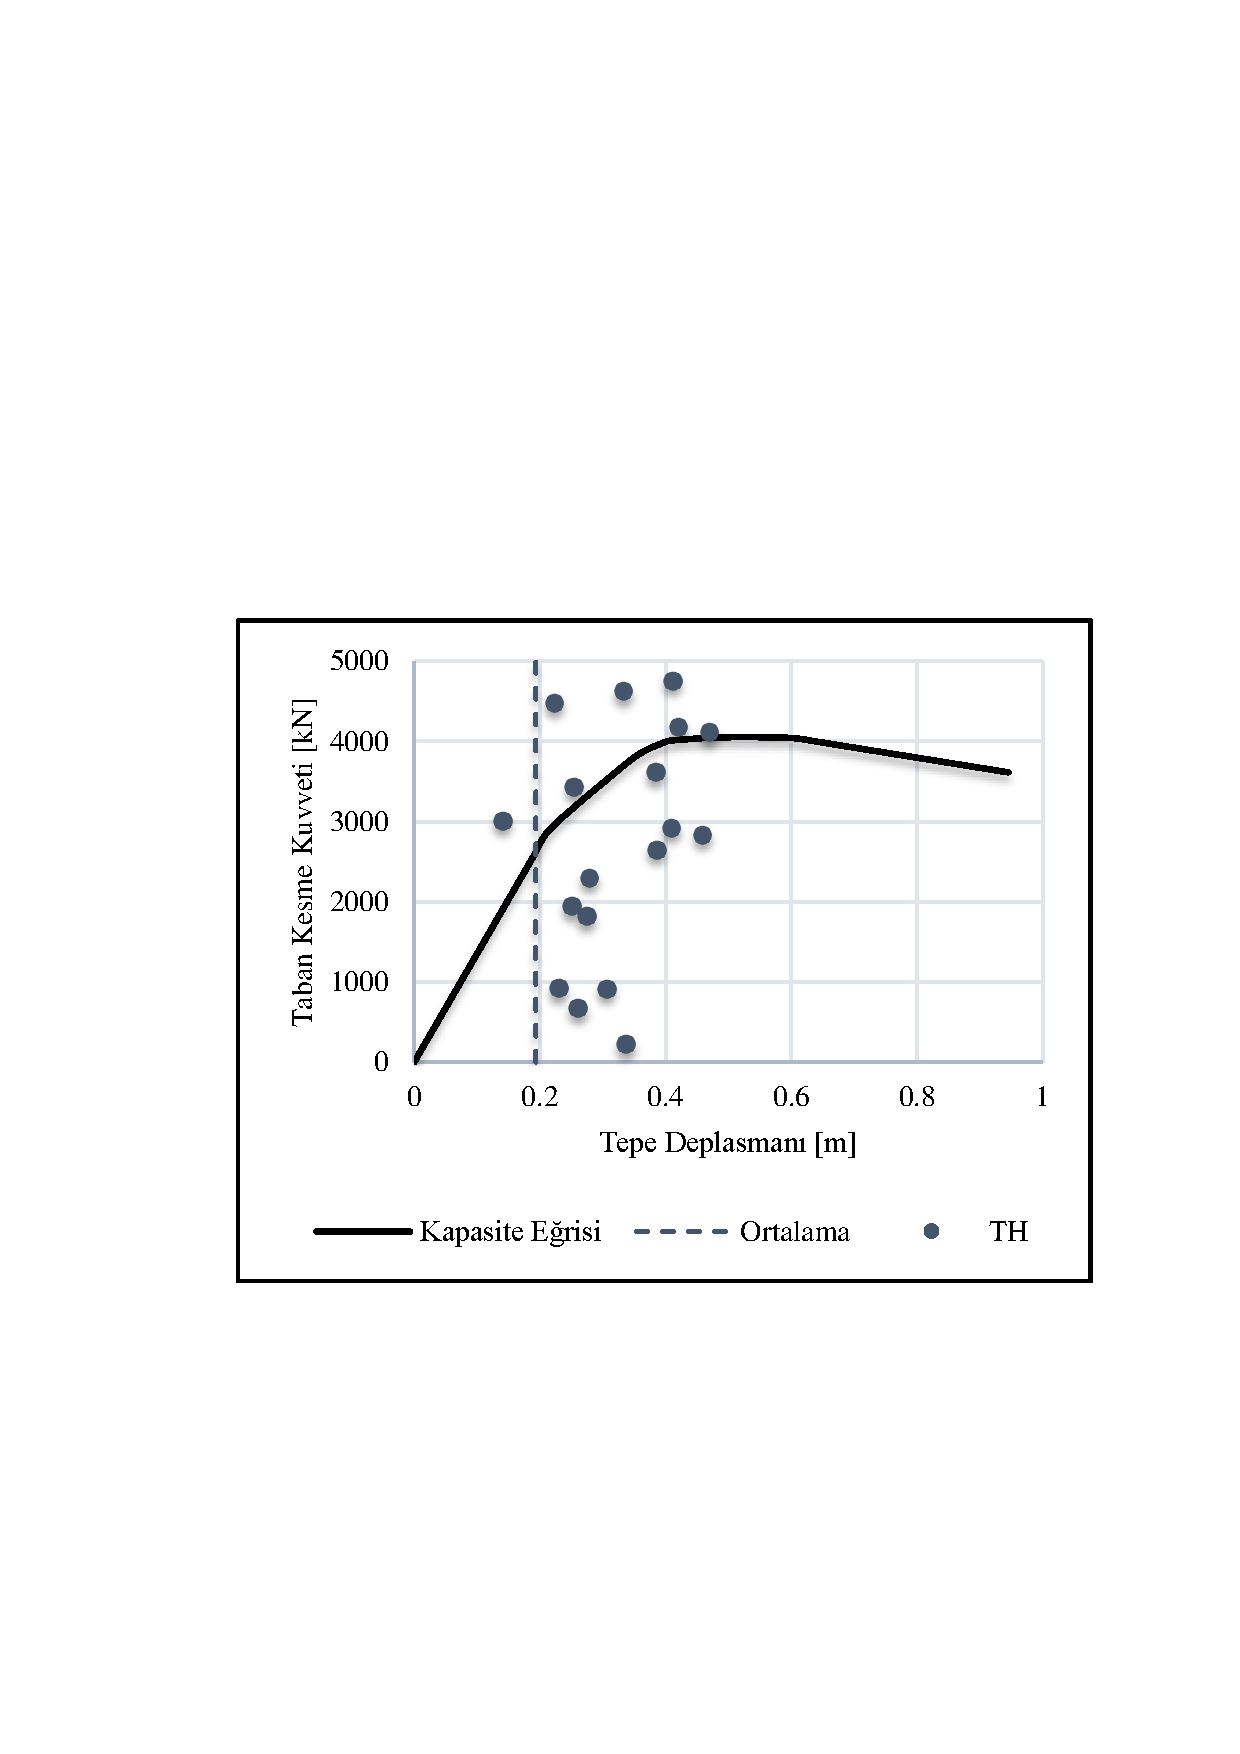
\includegraphics[width=6.5cm,height=6cm]{TikZ/Grafik_1}\hspace{1cm}
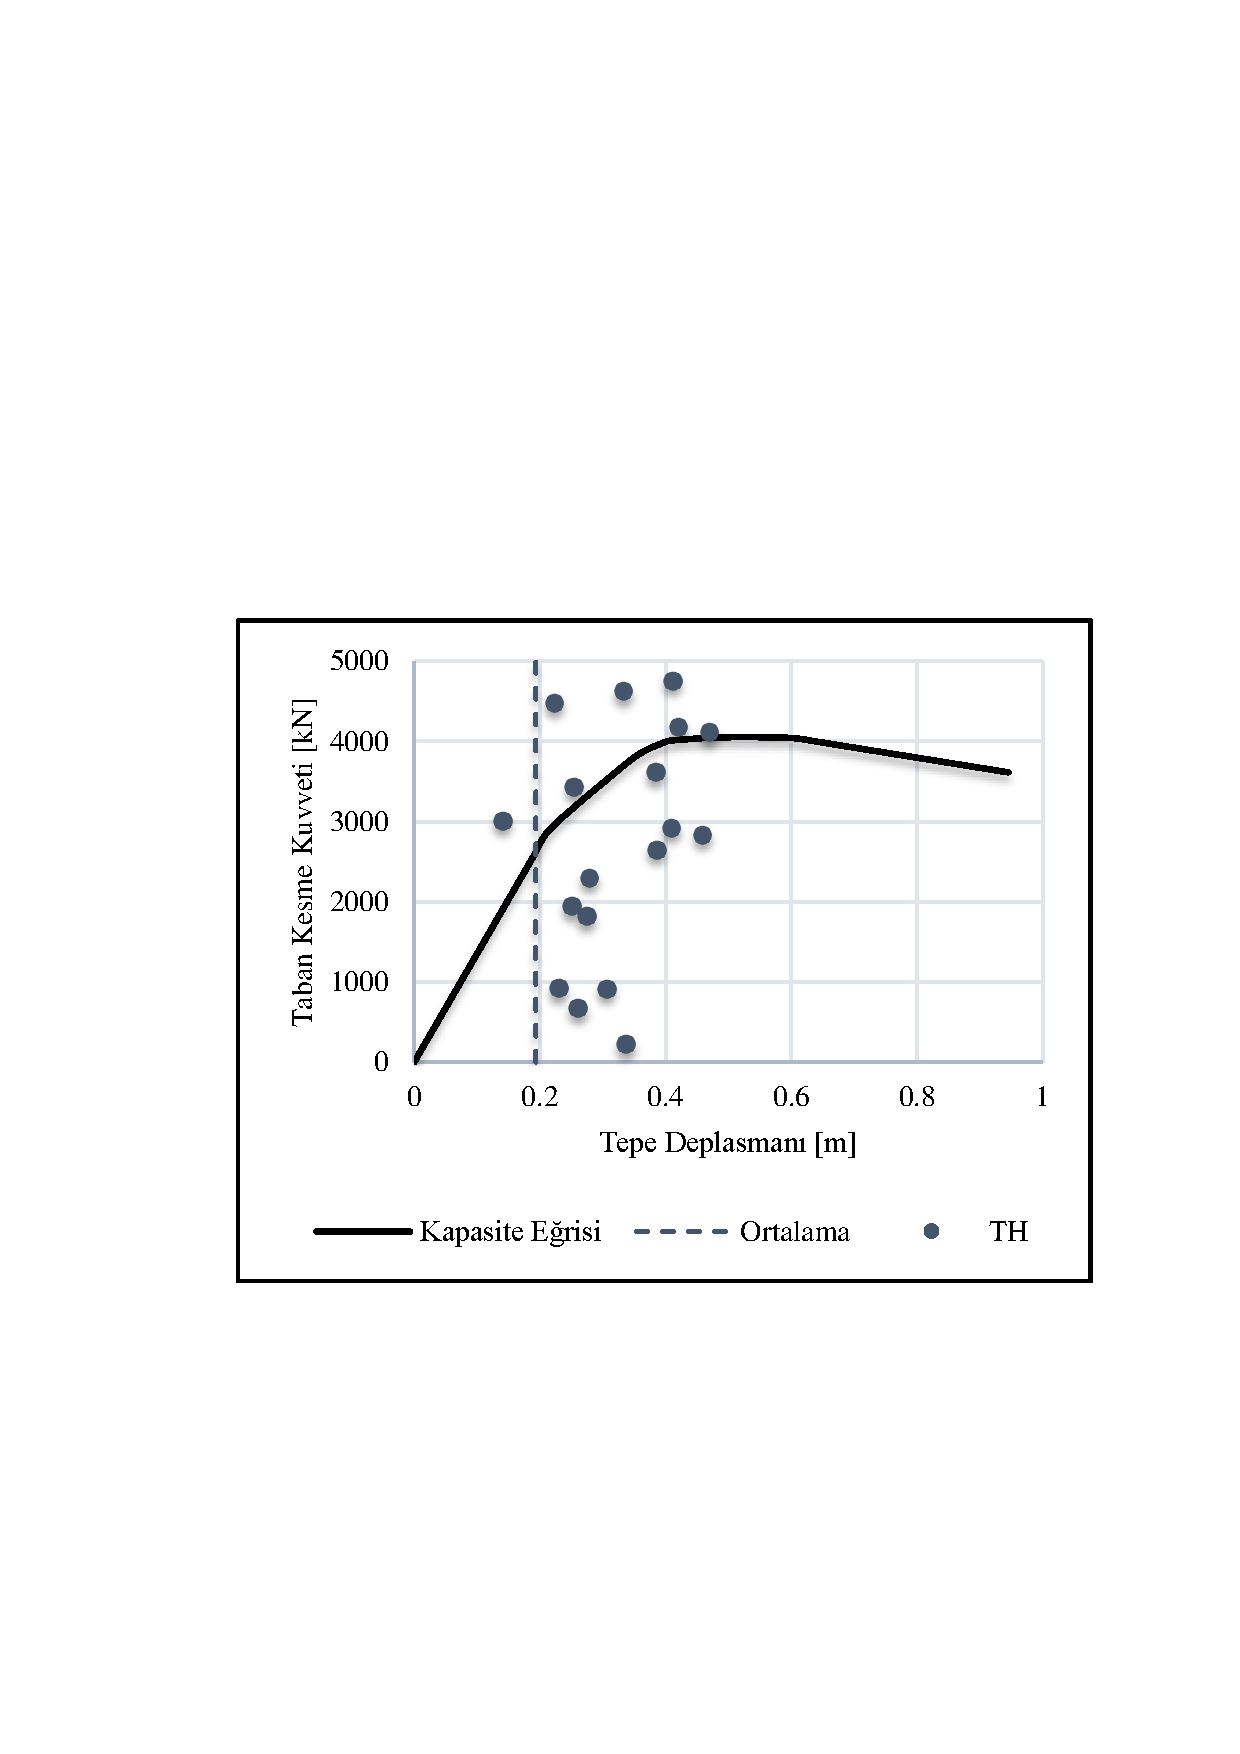
\includegraphics[width=6.5cm,height=6cm]{TikZ/Grafik_1}\caption{\label{fig:LRBIsolator} Kurşun çekirdekli kauçuk izolatör.}
\end{figure}

Yapıların mesnetleri üzerinde sarkaç gibi hareket etmelerini sağlayan
sismik yalıtım yöntemi Zayas ve diğerleri tarafından 1990 yılında
yapılan çalışmalar neticesinde önerilmiştir \cite{doi:10.1193/1.1585573}.
Şekil \ref{fig:FPIsolator}'de kesiti verilen sürtünmeli sarkaç tipi
izolatörlerin yalıtım periyotları konkav yüzeyin yarıçapı ile belirlenmektedir.
Deprem enerjisinin sönümlendiği histeretik davranış, yüzeylerde oluşan
sürtünme kuvvetleri nedeniyle oluşmaktadır. Sistemin sarkaç hareketine
başlaması, sürtünme kuvvetlerinin aşılmasıyla mümkün olmaktadır. Bu
nedenle yapının rüzgar yükleri altında yalıtım birimlerinden beklenen
rijitlik elde edilmiş olmaktadır. Sürtünmeli sarkaç tipi izolatörlerin
malzeme belirsizliklerinden en az düzeyde etkilenmesi, sismik yalıtımlı
yapıların deprem etkileri altındaki davranışlarının öngörülebilir
olmasını sağlamaktadır. Ayrıca yapılan testlere göre büyük deplasmanlarda
eksenel taşıma kapasitesinde düşme veya stabilite kaybı olmadığı ve
histeretik çevrimler ile dayanım azalmasının oluşmadığı görülmüştür.
\begin{figure}[h!]
\centering{}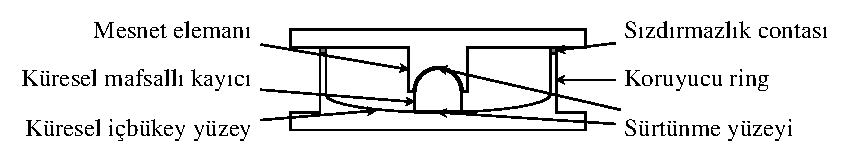
\includegraphics{TikZ/FPIsolator} \caption{\label{fig:FPIsolator}Sürtünmeli sarkaç tipi izolatör.}
 
\end{figure}

Sismik izolasyon, dünyada depremselliği yüksek olan bölgelerde yoğun
olarak kullanılmaktadır. Japonya, Çin, Rusya, İtalya ve ABD başta
olmak üzere 30 dan fazla ülkede 23.000'i aşkın bina, sismik izolasyon
ve sönümleyiciler ile korunmaktadır \cite{Martelli2014}. Aktif fay
hatları üzerinde bulunan ülkemizde ise sismik izolasyon kullanımı
giderek yaygınlaşmaktadır. Ağırlıklı olarak depremden hemen sonra
kesintisiz kullanımın hedeflendiği hastaneler ve veri merkezleri gibi
önemli binalarda uygulanmaktadır. İstanbul'da bulunan Sabiha Gökçen
Uluslararası Havalimanında üç sürtünme yüzeyli sarkaç tipi izolatörler
kullanılarak sismik yalıtım uygulanmıştır. Toplamda 160.000 $\mathrm{m^{2}}$'den
fazla alana kurulu havalimanında 252 sismik izolatör bulunmaktadır.
Üç sürtünme yüzeyli sismik izolatörler ve çelik üst yapının montajı
2008'de tamamlanmıştır (Şekil \ref{fig:SabihaG=0000F6k=0000E7en}).
\begin{figure}[h!]
\centering{}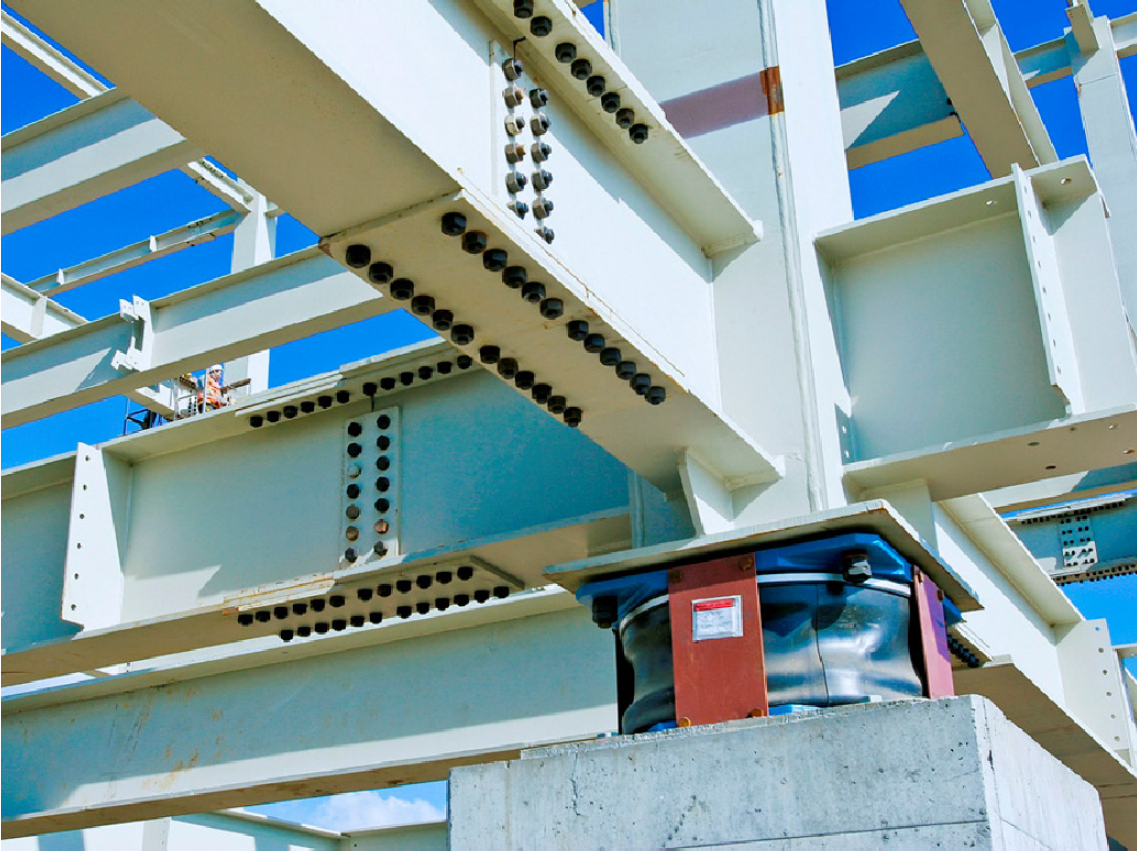
\includegraphics[height=5cm]{fig/a.PNG} \hspace{1cm}
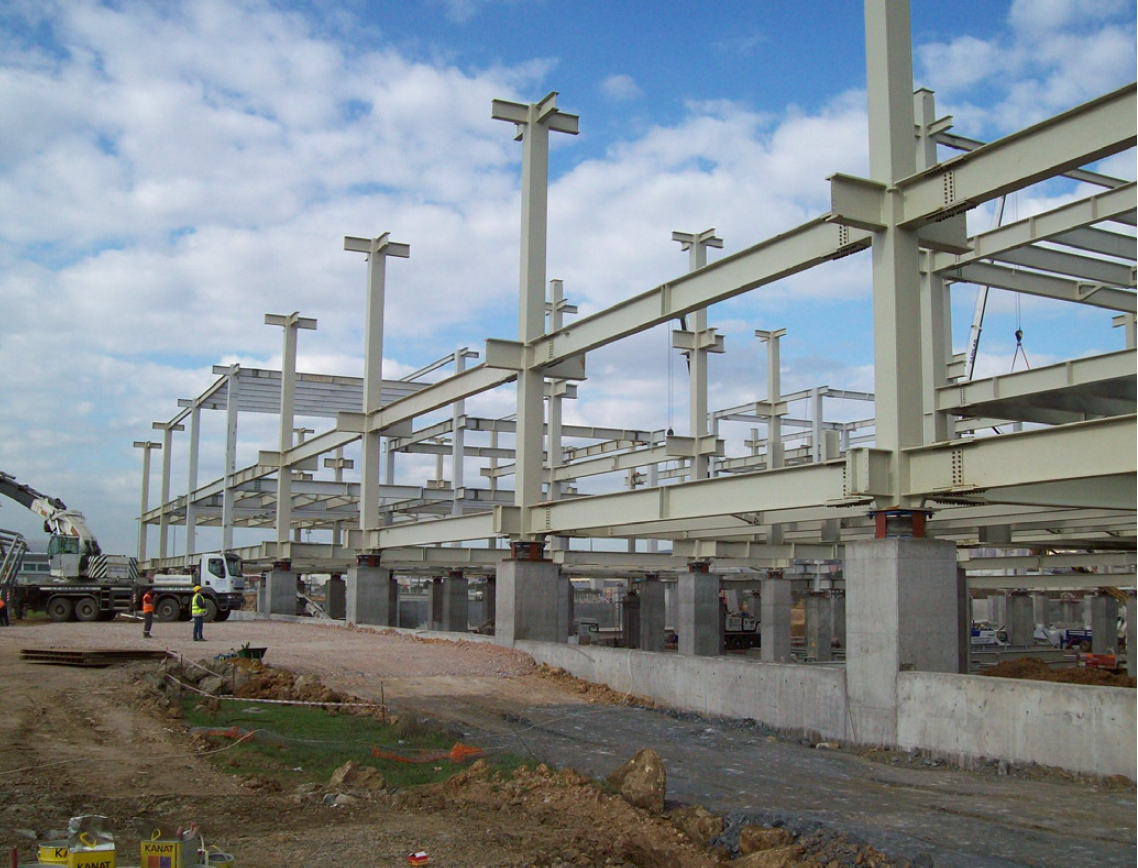
\includegraphics[height=5cm]{fig/b.PNG} \vspace{6pt}
 \caption{\label{fig:SabihaG=0000F6k=0000E7en} Sabiha Gökçen Uluslararası Havalimanına
ait sismik izolatör kolon kiriş birleşimi ve çelik üst yapı \cite{Zekioglu2009}.}
\end{figure}

\newpage{}

\section{Problemin Tanımı}

Sismik yalıtımlı yapıların tasarımı, doğrusal yöntemlerle ön boyutlandırma
aşaması ve doğrusal olmayan dinamik analizlerle tasarımın doğrulanması
olmak üzere iki aşamalıdır. Ön tasarım aşamasında eşdeğer doğrusal
analiz ve mod birleştirme yöntemleri kullanılmaktadır.

Sismik yalıtımlı yapılarda izolatörlerin hakim frekansları ile tabanı
ankastre kabul edilen üst yapı frekansları belirgin biçimde ayrıklaşır.
Göreli olarak düşük yatay rijitliğe sahip yalıtım birimleri, üst yapının
yapacağı deformasyonları azaltmaktadır. Bu nedenlerle elastik sınırlar
içerisinde davranması beklenen yapının, yapısal düzensizliklerinin
bulunmaması halinde gerekli idealleştirmeler yapılarak sistem basitleştirilebilir.
Ayrıca yapının sahip olduğu doğrusal olmayan dinamik özellikler, idealleştirilmiş
sisteme karşılık gelen parametrelerle ifade edilebilir. Eşdeğer doğrusal
analiz yönteminde tüm yapı, Şekil \ref{fig:equivalentmodel}'de belirtildiği
gibi tek serbestlik dereceli bir sistem olarak temsil edilmektedir.
\begin{figure}[h!]
\centering{}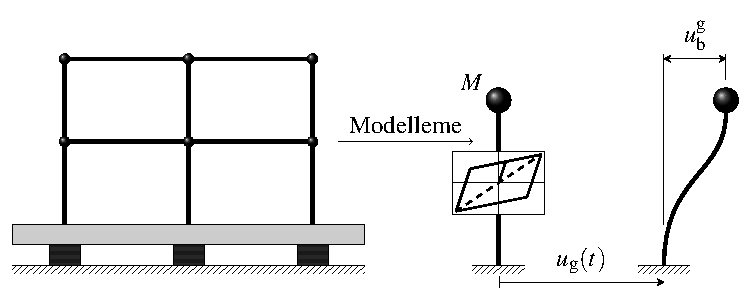
\includegraphics{TikZ/StructuralEquivalentModel} \caption{\label{fig:equivalentmodel} Eşdeğer Tek Serbestlik Dereceli Sistem.}
\end{figure}

Sismik yalıtımlı yapı sisteminin, tasarlanacağı yönetmelikte eşdeğer
doğrusal analiz için belirtilen uygulama sınırları dışında kalması
durumunda veya üst yapı taşıyıcı sisteminin sahip olduğu serbestlik
dereceleri de dikkate alınarak daha detaylı bir çözüm yapılmak istendiğinde
mod birleştirme yöntemi tercih edilmektedir. Üst yapının çok serbestlik
dereceli sistem olarak modellendiği bu yöntemde, izolatörlerin temsil
edildiği doğrusal kesme yaylarında eşdeğer rijitlik değerleri kullanılmaktadır.
Böylece kütlesi ve rijitliği belli olan sistemin doğrusal mod şekilleri
ve bu modlara karşılık gelen periyot ve frekans değerleri hesaplanır.
Tüm modlardan elde edilen iç kuvvet ve yer değiştirmeler birleştirilerek
sistemin deprem etkileri hesaplanır.

Doğrusal yöntemlerle tasarımı tamamlanan sismik yalıtımlı yapıların
kontrolü, geçmiş depremlerden elde edilen veya bölgenin depremsellik
özelliklerine uygun biçimde yapay olarak üretilen yer ivmeleri etkisinde,
yapıların doğrusal olmayan davranışlarının modellendiği, zaman tanım
alanında yapılan analizler ile sağlanır. İzolatör birimleri için kullanılan
kesme yaylarında doğrusal olmayan davranışların çeşitli malzeme modelleri
ile ifade edilebileceği gibi, eksenel yaylar, eğilme ve burulma yayları
da tanımlanabilmektedir. Ayrıca bu yayların birbirleri ile bağlı olarak
çalışması gerçeğe daha yakın analiz sonuçlarının elde edilmesini sağlamaktadır.
Bu analizde yapısal davranışlar, kütle ve rijitliklerin yanında yer
hareketlerinin içeriğine de bağlı olarak değişkenlik göstermektedir.
Bu nedenle yapının doğrusal olmayan dinamik analizinde, tasarımda
uyulan yönetmelik koşullarında belirtilen sayıda ve tasarım spektrumuna
göre ölçeklenmiş veya eşlenmiş yer ivmesi kullanılarak bulunan sonuçların
ortalaması değerlendirilmektedir.

Sismik yalıtımlı yapıların tasarım metotları 1970'lerden günümüze
kadar fiziksel deneyler veya analitik modellerden elde edilen bilgiler
ışığında pek çok kez irdelenmiştir. Yapılan araştırmalar içinde doğrusal
tasarım metotlarının geçerliliği, kullanım sınırları ve doğruluk mertebeleri
incelenen konular arasında bulunmaktadır. Sismik yalıtımlı yapıların
tasarımında kullanılan doğrusal yöntemler, konvansiyonel yapılardan
farklı olarak yalnızca ön tasarım aşamasında kullanılmaktadır. Öngörülen
en büyük depremden sonra dahi yapının kesintisiz olarak kullanılma
gerekliliği, yapısal tasarımda gerçeğe en yakın sonuçların elde edilmesini
sağlayacak analizlerin uygulanma zorunluluğunu da beraberinde getirmektedir.
Dolayısıyla ana hatları doğrusal analizler ile belirlenen sismik yalıtımlı
sistem tasarımlarının, bölgenin depremselliğine uygun olarak seçilecek
deprem kayıtları kullanılarak yapılacak doğrusal olmayan dinamik analizler
sayesinde kontrol edilerek son hale getirilmesi önemlidir. Fakat bu
ileri seviye analizler, karmaşık olabilmekte ve uzun zaman almaktadır.
Bu nedenle, son aşamaya kadar doğrusal yöntemler ile ilerletilen sismik
yalıtımlı yapı projelerinde bu analizlerin doğruluğu önem arz etmektedir.
İlerleyen başlıklarda doğrusal analiz yöntemleri irdelenmiştir.

\section{Amaç ve Kapsam}

\label{EquivalentLinearAnalysis} Eşdeğer doğrusal analiz yönteminde
kullanılan sistemde izolatörlerin üzerinde bulunan yalıtım düzlemi
ve üst yapı, tek bir kütle olarak değerlendirilmektedir. İzolatör
eşdeğer rijitliği, her bir izolatör biriminin tasarım deplasmanı için
elde edilecek sekant rijitlikleri toplamını belirtmektedir. Buna bağlı
olarak izolatör periyodu, tek serbestlik dereceli sistem için hesaplanmaktadır.
Sistemin sönümleyeceği enerji ise izolatörlerin doğrusal olmayan histeretik
davranışlarından elde edilecek eşdeğer viskoz sönüm oranı cinsinden
ifade edilir. Eşdeğer doğrusal analiz yöntemi, içerdiği kabul ve idealleştirmeler
sebebi ile kullanılan yönetmeliklerde belirtilen kriterlerin sağlanması
durumunda uygulanabilmektedir.

Ön tasarım aşamasında izolatörlerde meydana gelecek en büyük yatay
yer değiştirme değerinin tespit edilmesi izolatör boyutlarının belirlenmesinde
önemli bir kriterdir. En büyük yer değiştirme değeri, en büyük izolatör
kuvvetinin eşdeğer rijitliğe bölümü ile bulunmaktadır. Fakat eşdeğer
rijitlik değerinin belirlenebilmesi, izolatörün en büyük yer değiştirme
değerinin bilinmesi ile mümkün olmaktadır. Ön tasarımın ilk adımında
oluşan bu belirsizlik, detayları Bölüm \ref{CH2}'de sunulan iterasyonlar
ile ortadan kaldırılmaktadır.

Üst yapının ön tasarımı için gerekli taban kesme kuvveti, bu yöntemde
yalıtım düzleminde oluşan kesme kuvvetine göre hesaplanmaktadır. Tasarımda
takip edilen yönetmeliğe bağlı olarak taban kesme kuvvetinin belirlenmesi
ve bu kuvvetin üst yapı katlarına dağıtılma biçimi farklılık göstermektedir.
EN 1998-1:2004'e göre, katlara etkiyen yatay kuvvetler eşdeğer periyot
ve sönüme göre hesaplanacak spektral ivmenin, ilgili kat kütlesi ile
çarpımından elde edilmektedir\cite{Eurocode2004}. Burada kat kütlelerinin
eşit olduğu kabulü yapılırsa kesme kuvvetlerinin katlara eşit miktarda
dağıtıldığı görülmektedir. Ayrıca yalıtım birimi seviyesinde meydana
gelen kesme kuvvetinin yapı kütlesine oranı ile üst yapı taban kesme
kuvvetinin üst yapı toplam kütlesine oranı eşit olmaktadır.

ASCE/SEI-7-10 (2010) ve TBDY (2018) yönetmeliklerinde yer alan formüle
göre taban kesme kuvveti, yalıtım seviyesinde oluşan kesme kuvvetine
eşit alınarak üst yapı katlarına üçgen formunda dağıtılmaktadır \cite{ASCE2010,TBDY2018}.

ASCE/SEI-41-13 (2014) ve ASCE/SEI-7-16 (2016) yönetmeliklerinde ise
yalıtım düzleminde oluşacak kesme kuvveti, yapı taban kesme kuvvetine
eşit olarak alınmamaktadır \cite{ASCE41-13,ASCE2016}. York ve Ryan
tarafından yapılan çalışma, eşdeğer viskoz sönüm oranının artması
halinde, yapı taban kesme kuvvetinin yalıtım düzleminde oluşan kesme
kuvvetine oranının da artacağını göstermektedir \cite{doi:10.1080/13632460802003751}.
Buna bağlı olarak önerilen formül, istatistiksel parametreyi temsil
eden katsayıda bulunan değişiklik ile birlikte bu güncel yönetmeliklerde
yer almaktadır. Elde edilen artırılmış taban kesme kuvveti ise katlara
çalışmada önerilen formülün güncel haline göre paylaştırılmaktadır.

TBDY (2018) yönetmeliğine göre hesaplanacak taban kesme kuvvetinde
belirlenecek deprem yükü azaltma katsayısı $R$, hedeflenecek kesintisiz
kullanım ve sınırlı hasar performans düzeyleri için dayanım fazlalığı
katsayısı $D$ ile eşit verilmektedir \cite{TBDY2018}. Benzer olarak
ASCE/SEI-7-10 (2010) yönetmeliğinde belirtilen formülde yer alan $R_{1}$
katsayısı, üst yapı yatay taşıyıcı sistemine bağlı olarak belirlenecek
$R$ katsayısının $3/8$'i alınarak hesaplanmakta ve en fazla $2$
olarak belirlenebilmektedir \cite{ASCE2010}. Dolayısıyla $R_{1}$
katsayısı, hiçbir taşıyıcı sistem için dayanım fazlalığı katsayısı
$\Omega_{\text{0}}$'dan büyük olmamaktadır. Böylece yapının karşılaşması
beklenen en büyük deprem etkisi altında elastik sınırlar içinde kalması,
yalnızca eşdeğer doğrusal analiz yönteminin belirlediği kabuller çerçevesinde,
yalıtım düzlemi kesme kuvvetinin üst yapı taban kesme kuvvetine eşit
olması durumunda mümkün olmaktadır.
